% Ubah judul dan label berikut sesuai dengan yang diinginkan.
\section{Tinjauan Pustaka}
\label{sec:tinjauanpustaka}

\subsection{Penelitian Terdahulu}
\label{subsec:penelitianterdahulu}

Penelitian yang dilakukan oleh Andi Aljabar dan Suhartijo berhasil menerjemahkan bahasa isyarat Indonesia dengan arsitektur Convolutional Neural Network (CNN), Long Short-Term Memory (LSTM), dan kombinasi keduanya. Pengujian dengan 10 kelas kosakata BISINDO menunjukkan akurasi rata-rata 73\% pada CNN, 81\% pada LSTM, dan 90\% pada gabungan CNN-LSTM \cite{aljabar2020}. Penelitian oleh Husna Moetia Putri, Fadlisyah, dan Wahyu Fuadi mendeteksi bahasa isyarat secara real-time menggunakan LSTM dan MediaPipe Holistic. Evaluasi pada 10 kosakata BISINDO mencapai akurasi 92\% dan pada 30 kosakata akurasi mencapai 65\% \cite{putri2022}. Siti Nur, Aghisna Nur Assyifa, dan Habilah Nurjannah mengembangkan aplikasi penerjemah BISINDO menggunakan LSTM dengan akurasi 75\% pada 500 data, meningkat menjadi 85\% pada 1000 dan 1500 data. Aplikasi ini memiliki fitur menambah kosakata dan menyimpan data untuk menghasilkan output kosakata isyarat yang sesuai \cite{nur2023}.

\subsection{Bahasa Isyarat Indonesia (BISINDO)}
\label{subsec:tunarungu}

Tunarungu adalah istilah untuk seseorang yang kehilangan atau tidak mampu menangkap rangsangan auditori melalui indra pendengarannya \cite{mursita2015}. Berdasarkan kelahiran, tunarungu dapat dibagi menjadi dua, yaitu \emph{congenitally deaf} (sejak lahir) dan \emph{adventitiously deaf} (karena penyakit atau peristiwa traumatis). Tunarungu juga diklasifikasikan berdasarkan tingkat kemampuan pendengaran dalam \emph{decibel} (dB), dari ringan hingga total \cite{winarsih2007}. Di Indonesia, terdapat setidaknya 2,9 juta atau 1,25\% penduduk yang merupakan penyandang tunarungu \cite{evitasari2015}. 
Penyandang tunarungu menggunakan bahasa isyarat dalam berkomunikasi. Bahasa isyarat adalah bahas yang diungkapkan dengan kombinasi antara bentuk tangan, orientasi dan gerak tangan, lengan tubuh, serta ekspresi wajah \cite{mursita2015}. Terdapat dua bahasa isyarat yang berkembang di Indonesia, yaitu Sistem Bahasa Isyarat Indonesia (SIBI) dan Bahasa Isyarat Indonesia (BISINDO). SIBI menggunakan satu tangan, sedangkan BISINDO menggunakan dua tangan. BISINDO lebih umum digunakan karena tidak terikat struktur bahasa Indonesia dan berasal dari bahasa ibu tunarungu dan menyesuaikan pemahaman mereka tanpa menekankan struktur imbuhan bahasa Indonesia.

\subsection{Mediapipe}
\label{subsec:mediapipe}
MediaPipe adalah kerangka kerja (\emph{framework}) untuk membangun \emph{pipeline} inferensi pada data sensorik seperti audio dan video. Framework ini memungkinkan pembuatan pipeline yang terdiri dari komponen modular, seperti model inferensi, algoritma pemrosesan media, dan transformasi data. MediaPipe mengabstraksikan dan menghubungkan model-model persepsi individu ke dalam alur yang dapat dipertahankan, sehingga komponen dapat digunakan kembali. Konsep dasar MediaPipe mencakup kerangka kerja inferensi data sensorik, alat evaluasi kinerja, dan komponen pemrosesan yang dapat digunakan kembali. MediaPipe dirancang untuk mendukung pengembangan model \emph{machine learning} dan \emph{deep learning}, seperti deteksi objek dan pendeteksian gerakan bahasa isyarat \cite{lugaresi2019:}. Mediapipe Pose merupakan \emph{framework} yang dapat memprediksi total 33 lokasi \emph{landmark}, dengan diawali dari bagian hidung hingga diakhiri pada kaki bagian kanan. Mediapipe Hand merupakan \emph{framework} yang dapat memprediksi 21 lokasi \emph{landmark} yang meliputi keseluruhan tangan \cite{googleMediapipe}.


\subsection{\emph{Long Short Term-Memory} (LSTM)}
\label{subsec:lstm}

\begin{figure}[ht]
    \centering

    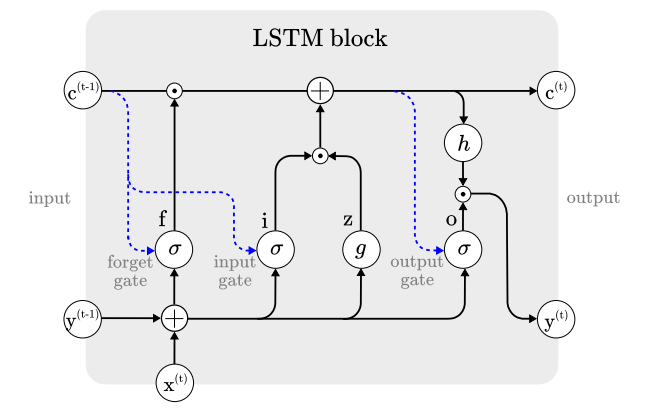
\includegraphics[scale=0.5]{gambar/bab2-lstm-model.png}
 
    \caption{Cara kerja arsitektur LSTM}
    \label{fig:longshortterm}
\end{figure}

\textit{Long Short-Term Memory} (LSTM) merupakan bentuk khusus dari neural network RNN atau \textit{Recurrent Neural Network} yang memiliki kemampuan \textit{feedback connection}. Kemampuan ini memungkinkan LSTM untuk dapat mengingat informasi untuk waktu yang lama sehingga dapat digunakan untuk menyelesaikan permasalahan yang memiliki sifat sekuensial atau berurutan. Keunggulan LSTM jika dibandingkan dengan RNN adalah LSTM memiliki kemampuan untuk mengingat informasi yang lebih baik dan efektif sehingga meminimalisir terjadinya kehilangan informasi yang umum terjadi pada pemrosesan informasi lama yang panjang pada penggunaan RNN \cite{xia2020}. LSTM sangat tepat digunakan untuk melakukan klasifikasi bahasa isyarat yang bersifat sekuensial. Pada gambar \ref{fig:longshortterm}, \textit{Long Short-Term Memory} tersusun atas beberapa layer yang meliputi \textit{block input}, \textit{input gate}, \textit{forget gate}, \textit{cell}, \textit{output gate}, dan \textit{block output} yang dapat dirumuskan secara berurutan sebagai berikut:

\begin{equation}
    \label{eq:blockinputLSTM}
    x^{(t)} = g(W_z x^{(t)} + R_z y^{(t-1)} + b_z)
  \end{equation}

  \begin{equation}
    \label{eq:inputgateLSTM}
    i^{(t)} = \sigma(W_i x^{(t)} + R_i y^{(t-1)}+ p_i \odot c^{(t-1)} + b_i)
\end{equation}

\begin{equation}
    \label{eq:cellLSTM}
    c^{(t)} =  z^{(t)} \odot  i^{(t)} + z^{(t-1)} \odot  f^{(t)}
\end{equation}

\begin{equation}
    \label{eq:outputgateLSTM}
    o^{(t)} = \sigma(W_o x^{(t)} + R_o y^{(t-1)}+ p_o \odot c^{(t)} + b_o)
\end{equation}

\subsection{Intel \emph{Next Unit Computing} (NUC)}
\label{subsec:intelNUC}

Intel \emph{Next Unit Computing} (NUC) merupakan komputer \emph{barebone} dengan ukuran kecil yang dirancang oleh Intel. Intel NUC merupakan perangkat yang berfokus dalam menyediakan komputasi kuat dalam ukuran yang praktis dan dapat melayani berbagai kebutuhan pengguna, mulai dari bermain \emph{game}, bisnis, hingga menjalankan aplikasi kompleks. Intel NUC secara resmi memperkenalkan perangkat ini pada tahun 2012 dan dipasarkan secara umum pada awal tahun 2013 \cite{IntelNUC2020}. Adapun seri pertama dari Intel NUC memiliki CPU Sandy Bridger berbasis Celeron. Intel NUC telah berkembang hingga generasi ke-12 bernama Dragon Canyon yang dilengkapi dengan CPU Intel generasi ke-12 dan PCI Express Gen 5 \cite{Halfacree2013}.

% Beberapa penelitian lain pernah dilakukan seperti yang dirumuskan oleh \citet{newton1687} bahwa \lipsum[5]
% Hasil tersebut kemudian menjadi persamaan \ref{eq:hukumpertama}.

% % Contoh pembuatan persamaan ilmiah.
% \begin{equation}
%   \label{eq:hukumpertama}
%   \sum \mathbf{F} = 0\; \Leftrightarrow\; \frac{\mathrm{d} \mathbf{v} }{\mathrm{d}t} = 0.
% \end{equation}

% \lipsum[6-7]